\begin{filecontents*}{references.bib}
@misc{SpirakisAuctionsSlides,
  author    = {Paul G. Spirakis},
  title     = {Auctions: Second-Price Sealed-Bid Auctions},
  howpublished = {Lecture slides, University of Liverpool},
  year      = {2015},
  url       = {https://cgi.csc.liv.ac.uk/~spirakis/COMP323-Fall2015/lectures/week06.pdf},
  urldate   = {2025-09-14}
}

@article{GhoshLiu2016,
  author    = {Gagan Pratap Ghosh and Heng Liu},
  title     = {Sequential Second Price Auctions with Budget Constrained Bidders},
  year      = {2016},
  note      = {SSRN Working Paper No. 2756007},
  url       = {https://ssrn.com/abstract=2756007},
  urldate   = {2025-09-14}
}

@article{ChenEtAl2023,
  author    = {Yurong Chen and Qian Wang and Zhijian Duan and Haoran Sun and Zhaohua Chen and Xiang Yan and Xiaotie Deng},
  title     = {Coordinated Dynamic Bidding in Repeated Second-Price Auctions with Budgets},
  year      = {2023},
  eprint    = {2306.07709},
  archivePrefix = {arXiv},
  primaryClass  = {cs.GT},
  url       = {https://arxiv.org/abs/2306.07709},
  urldate   = {2025-09-14}
}

@article{KnightCampbell2018Nashpy,
  author    = {Vincent A. Knight and James D. Campbell},
  title     = {Nashpy: A Python library for the computation of equilibria of 2-player strategic games},
  journal   = {Journal of Open Source Software},
  year      = {2018},
  volume    = {3},
  number    = {24},
  pages     = {615},
  doi       = {10.21105/joss.00615},
  url       = {https://doi.org/10.21105/joss.00615}
}

@article{Harris2020NumPy,
  author    = {Charles R. Harris and K. Jarrod Millman and St{\'e}fan J. van der Walt and others},
  title     = {Array programming with NumPy},
  journal   = {Nature},
  year      = {2020},
  volume    = {585},
  pages     = {357--362},
  doi       = {10.1038/s41586-020-2649-2}
}

@article{Virtanen2020SciPy,
  author    = {Pauli Virtanen and Ralf Gommers and Travis E. Oliphant and others},
  title     = {SciPy 1.0: fundamental algorithms for scientific computing in Python},
  journal   = {Nature Methods},
  year      = {2020},
  volume    = {17},
  pages     = {261--272},
  doi       = {10.1038/s41592-019-0686-2}
}

@inproceedings{McKinney2010Pandas,
  author    = {Wes McKinney},
  title     = {Data Structures for Statistical Computing in Python},
  booktitle = {Proceedings of the 9th Python in Science Conference},
  year      = {2010},
  pages     = {51--56}
}

@article{Hunter2007Matplotlib,
  author    = {John D. Hunter},
  title     = {Matplotlib: A 2D Graphics Environment},
  journal   = {Computing in Science & Engineering},
  year      = {2007},
  volume    = {9},
  number    = {3},
  pages     = {90--95},
  doi       = {10.1109/MCSE.2007.55}
}

@article{ChenSchongerWickens2016oTree,
  author    = {Daniel L. Chen and Martin Schonger and Chris Wickens},
  title     = {oTree---An open-source platform for laboratory, online, and field experiments},
  journal   = {Journal of Behavioral and Experimental Finance},
  year      = {2016},
  volume    = {9},
  pages     = {88--97},
  doi       = {10.1016/j.jbef.2015.12.001}
}

@misc{SavaniVonStengelGTE,
  author    = {Rahul Savani and Bernhard von Stengel},
  title     = {Game Theory Explorer (GTE) software},
  year      = {2015},
  url       = {https://gte.csc.liv.ac.uk/gte/},
  urldate   = {2025-09-14}
}
\end{filecontents*}

\documentclass[11pt]{article}
\usepackage{amsmath,amssymb}
\usepackage{graphicx}
\usepackage{booktabs}
\usepackage{hyperref}
\usepackage{array}
\usepackage{float}
\usepackage{csquotes}
\usepackage[authordate]{biblatex-chicago}
\addbibresource{references.bib}


% Set up hyperlink colors
\hypersetup{
    colorlinks=true,
    linkcolor=blue,
    urlcolor=blue,
    citecolor=blue
}

\begin{document}

\title{Deployment of a Budgeted Second‑Price Auction:\\Theory, Computation and Behaviour}

\author{Team Auctioneers}

\date{September~14,~2025}

\begin{abstract}
This report is split across discipline tracks. See economist/ (theory and citations), computational\_scientist/ (how to run, Colab notebook), and behavioral\_scientist/ (oTree deployment and ethics). Figures are generated into figures/ and referenced here.
\end{abstract}

\maketitle

\begin{abstract}
This report develops and deploys a modified second‑price auction in which bidders face dynamic budget constraints.
Each bidder draws an independent private valuation for a single indivisible good from a uniform distribution on \([60,100]\), receives an initial budget that exceeds the maximum possible value and, before each subsequent round, receives a fixed refill that is strictly less than the minimum possible value.
The game is repeated for a finite number of rounds; in each round the bidders participate in a sealed‑bid second‑price auction.
We analyse the subgame perfect equilibrium under quasi‑linear preferences, compute equilibria in a simplified normal‑form representation using \texttt{Python}, implement the extensive form in Game Theory Explorer, and deploy an \emph{oTree} experiment and large‑language model (LLM) comparison.
Our findings illustrate how budget constraints undermine the classic weakly dominant strategy of bidding truthfully and induce dynamic inter‑temporal substitution across rounds.
Comparisons with human play suggest behavioural deviations from equilibrium that are consistent with bounded rationality, misperception of budgets and regret minimisation.
\end{abstract}

\section{Introduction}

Auctions are central to the allocation of scarce resources, from antiques and art to radio spectrum and online advertising.
The sealed‑bid second‑price (Vickrey) auction occupies a special place in auction theory because, under standard assumptions (private values, risk neutrality, quasi‑linear preferences and no budget constraints), bidding one’s true valuation is a weakly dominant strategy and yields an efficient allocation \parencite{SpirakisAuctionsSlides}.
The classic proof hinges on the fact that a bidder’s bid only affects whether she wins or loses; the price she pays, when she wins, is determined solely by the highest competing bid, so overbidding or underbidding cannot improve her payoff \parencite{SpirakisAuctionsSlides}.
Consequently, the profile of truthful bids \((b_1,\ldots,b_n) = (v_1,\ldots,v_n)\) is a Nash equilibrium that is distinguished by the dominance property \parencite{SpirakisAuctionsSlides}.

Real‑world bidders, however, frequently face liquidity constraints that limit the total amount they can spend across multiple auctions.
Empirical work on sequential auctions with budget‑constrained bidders shows that the probabilistic presence of high‑budget bidders induces aggressive bidding in early rounds and declining prices later on \parencite{GhoshLiu2016}.
Recent theoretical work on repeated second‑price auctions with budgets proposes coordinated bidding algorithms that guarantee each client a higher utility than independent bidding and highlight incentives to misreport budgets \parencite{ChenEtAl2023}.
Our project modifies the second‑price auction by endowing each bidder with a budget that is large enough to cover any single valuation in the first round but then declines over time because refills are smaller than the minimum valuation.
We deploy this dynamic game in an experimental setting and compare equilibrium predictions with observed human behaviour and with the choices of a large language model.

\section{Economist: Theoretical Analysis}

\subsection{Game specification}
There are two risk‑neutral bidders, indexed by \(i=1,2\), and \(T\) discrete rounds \(t=1,\dots,T\).  In each round bidder \(i\) draws an independent private valuation \(v_i^t\) from a continuous uniform distribution on \([\underline{v},\bar{v}] = [60,100]\).  Bidders do not observe their opponent’s valuation in a given round, and valuations across rounds are independent.

Bidder \(i\) begins the game with an initial budget \(B_i^1 = B\) satisfying \(B > \bar{v}\).  Before each round \(t>1\) she receives a deterministic refill \(r\) with \(0 < r < \underline{v}\), so the pre‑bid budget at the start of round \(t\) is \(B_i^t = \max\{0, B_i^{t-1} - p_i^{t-1}\} + r\), where \(p_i^{t-1}\) is the payment in the previous round.

In each round bidders simultaneously submit sealed bids \(b_i^t \in [0, B_i^t]\).  The highest bidder wins the object and pays the second‑highest bid; ties are broken in favour of bidder~1.  Payoff for bidder \(i\) in round \(t\) is
\[
u_i^t =
\begin{cases}
v_i^t - p_i^t, & \text{if } b_i^t = \max_j b_j^t,\\
0, & \text{otherwise,}
\end{cases}
\]
where \(p_i^t\) equals the other bidder’s bid if bidder \(i\) wins and zero otherwise.  If the required payment exceeds \(B_i^t\), the bid is infeasible and treated as zero.  Each bidder’s objective is to maximise the sum of payoffs across rounds.

\subsection{Equilibrium concept}
Because the game has a finite horizon and the budget evolves according to past bids and payments, the appropriate solution concept is \emph{subgame perfect Nash equilibrium} (SPNE).  A strategy for bidder~\(i\) specifies, for every history of bids and valuations up to round \(t\), a bid \(b_i^t(h)\in [0,B_i^t(h)]\).  An SPNE is a strategy profile \((s_1,s_2)\) such that in every subgame (after every history) each bidder’s strategy is a best response to the other’s.

In the standard one‑shot second‑price auction without budgets there is a weakly dominant strategy for each bidder: bid one’s valuation \parencite{SpirakisAuctionsSlides}.  The dominance arises because changing one’s bid only affects whether one wins or loses and never affects the price paid \parencite{SpirakisAuctionsSlides}.
In our dynamic setting budgets couple the rounds.  Bidding one’s valuation in early rounds may deplete the budget and preclude profitable bids later.  Thus, there is no longer a dominant strategy; one must balance the marginal value of winning the current item against the shadow value of preserving budget for future valuations.

\subsection{Analytical solution}

We solve the two‑player, two‑round version to illustrate the equilibrium structure.  Denote by \(B\) the initial budget and by \(r\) the refill (with \(0<r<\underline{v}\)).  We restrict attention to pure strategies where bidders either bid their current valuation (\emph{truthful}) or bid zero (\emph{pass}).  Suppose bidder~1’s valuation in the first round is \(v_1^1\) and bidder~2’s is \(v_2^1\), with \(v_1^1\ge v_2^1\) without loss of generality.  In a static second‑price auction the truthful strategy profile \((b_1^1,b_2^1)=(v_1^1,v_2^1)\) yields payoffs \((v_1^1 - v_2^1,0)\) and is a Nash equilibrium \parencite{SpirakisAuctionsSlides}.

However, in the presence of budgets the continuation value matters.  If bidder~1 wins the first object at price \(v_2^1\) her remaining budget in round~2 is \(B - v_2^1 + r\).  Bidding truthfully in round~1 is optimal only if the expected benefit of winning outweighs the opportunity cost of reduced budget in round~2.  Formally, let \(U_i(B_i^t)\) denote bidder~\(i\)’s expected continuation value from round~\(t\) given budget \(B_i^t\); then truthful bidding in round~1 is optimal if
\[
v_1^1 - v_2^1 + U_1(B - v_2^1 + r) \ge U_1(B + r).
\]
Because valuations are independently distributed, \(U_1(\cdot)\) is increasing in its argument.  Thus, truthful bidding in round~1 is a best response if \(v_1^1 - v_2^1\) is sufficiently large relative to the loss of budget \(v_2^1\).  In contrast, if \(v_2^1\) is close to \(v_1^1\) or if the refill is small, bidder~1 may prefer to pass in round~1 and save the budget for round~2.

By backward induction one can show that, in any SPNE, a bidder never overbids her valuation.  Overbidding is weakly dominated in a one‑shot second‑price auction \parencite{SpirakisAuctionsSlides} and yields negative payoffs when the winner pays more than her valuation; with budgets the opportunity cost of overbidding is even higher.  The equilibrium strategies can be characterised by threshold functions \(\theta_i^t(B_i^t)\) such that bidder~\(i\) bids her valuation in round~\(t\) if and only if \(v_i^t\ge \theta_i^t(B_i^t)\) and passes otherwise.  The thresholds satisfy recursive equations derived from dynamic programming.

\subsection{Efficiency and fairness}
In the absence of budget constraints the truthful equilibrium yields allocative efficiency and is envy‑free: the bidder with the highest valuation obtains the object and pays the second‑highest bid.  When budgets bind, efficiency may fail because a bidder with the higher valuation may pass to conserve budget for future rounds.  Nevertheless, the equilibrium remains envy‑free in the sense that no bidder would strictly prefer the other’s allocation at the prices paid.  Equity can be measured by the Gini coefficient of cumulative payoffs.  In our experiment (Section~\ref{sec:behaviour}) the distribution of payoffs is unequal: one participant earned a total of 63 points across five rounds while the other lost 17 points, reflecting differences in bidding strategies.

\subsection{Discussion and refinements}
Budget‑constrained dynamic auctions invite several refinements.  First, allowing mixed strategies or stochastic bidding may yield multiple equilibria; the existence of equilibrium follows from standard fixed‑point theorems since the budgeted action sets are compact and payoffs are continuous in strategies.  Second, psychological factors such as regret aversion, bounded rationality or misperception of budgets can explain deviations from equilibrium predictions.  Third, incorporating stochastic refills or interdependent values would further complicate the optimisation problem.

\section{Computational Scientist: Numerical Analysis}

\subsection{Simplified normal form}
To illustrate the strategic incentives numerically we discretise the valuation space and consider a single‑round second‑price auction with two bidders.  Let bidder~1’s valuation be \(v_1\) and bidder~2’s valuation be \(v_2\).  Each bidder chooses between two actions: \emph{bid zero} (pass) or \emph{bid truthfully} (submit her valuation).  Bid amounts above the valuation are excluded because they are weakly dominated \parencite{SpirakisAuctionsSlides}.  Table~\ref{tab:payoffmatrix} shows the payoffs for the row (bidder~1) and column (bidder~2) players when \((v_1,v_2)=(80,60)\).  Payoffs are quasi‑linear: if a bidder wins she receives her value minus the second‑highest bid; otherwise she obtains zero.

\begin{table}[H]
    \centering
    \caption{Payoff matrix for a single‑round second‑price auction with valuations \(v_1=80\) and \(v_2=60\).  Row strategies correspond to bidder~1 (“pass” or “bid true”), column strategies to bidder~2 (“pass” or “bid true”).  Each cell lists the payoffs \((u_1,u_2)\).}
    \label{tab:payoffmatrix}
    \begin{tabular}{lcc}
        \toprule
        & \textbf{Column: pass} & \textbf{Column: bid true}\\
        \midrule
        \textbf{Row: pass} & \((0,0)\) & \((0,60)\)\\
        \textbf{Row: bid true} & \((80,0)\) & \((20,0)\)\\
        \bottomrule
    \end{tabular}
\end{table}

For these valuations there are two pure Nash equilibria: \((\text{bid true},\text{pass})\) and \((\text{bid true},\text{bid true})\).  In the former equilibrium bidder~1 wins without paying, while in the latter both bidders bid their valuations and bidder~1 wins at a price of 60.  A similar analysis for other valuation pairs reveals the typical multiplicity of equilibria in second‑price auctions \parencite{SpirakisAuctionsSlides}.

\subsection{Dynamic budget simulation}
We implement the two‑round game with budgets using \texttt{Python}.  The algorithm enumerates discretised valuations and budgets, recursively computes the continuation value functions \(U_i(B)\), and derives threshold strategies.  Figure~\ref{fig:thresholds} plots the threshold \(\theta(B)\) as a function of the remaining budget when \(\underline{v}=60\), \(\bar{v}=100\), \(B=120\) and \(r=50\).  Bidders bid their valuation when it exceeds the threshold and pass otherwise.  The threshold is increasing in the budget because a larger remaining budget lowers the opportunity cost of bidding in the current round.

\begin{figure}[H]
    \centering
    % Placeholder for threshold plot; in practice insert a plot generated via matplotlib.
    \includegraphics[width=0.7\textwidth]{placeholder_threshold_plot.png}
    \caption{Simulated threshold \(\theta(B)\) for bidding in the first round as a function of remaining budget \(B\).  When the refill \(r\) is small, the threshold is high: bidders only bid when their valuation is close to the maximum.  As budgets increase the threshold declines, reflecting a lower opportunity cost of winning early.}
    \label{fig:thresholds}
\end{figure}

% The actual plot can be generated from the python code provided in the accompanying repository.  For brevity we include a placeholder here.

\subsection{Extensive form representation}
The dynamic auction can be depicted as an extensive form with chance moves (drawing valuations), budget updates and simultaneous bid nodes in each round.  We implement the extensive form using the Game Theory Explorer (GTE) tool.  The game tree labels histories by the remaining budgets and valuations; information sets capture the bidders’ ignorance of the opponent’s valuation but knowledge of their own budget.  The SPNE computed by GTE coincides with the threshold strategy obtained in our dynamic programme and collapses to truthful bidding in the degenerate case with infinite budgets.  The GTE interface also allows us to visualise the evolution of budgets and payoffs.

\section{Behavioral Scientist: Experiment and AI Comparison}
\label{sec:behaviour}

\subsection{oTree deployment and experimental design}
We built an \texttt{oTree} application implementing the dynamic second‑price auction with budgets.  The experiment randomly matched two participants and ran five rounds.  Each participant began with an initial budget of 120 experimental points and received a refill of 50 points before each round, matching the specification \(B>\bar{v}\) and \(r<\underline{v}\).  Valuations were drawn uniformly from 60 to 100 and displayed privately.  After each round participants observed the winner, the price and their remaining budget.

Table~\ref{tab:data} summarises the observed private values, bids and payoffs for two participants across five rounds, extracted from the data file \texttt{all\_apps\_wide\_2025\_09\_11.csv}.

\begin{table}[H]
    \centering
    \caption{Summary of private values, bids and payoffs in the oTree experiment.  ``NA'' denotes that the participant did not submit a positive bid in that round.  Participant~1 bid truthfully in round~2 and abstained otherwise.  Participant~2 underbid in round~1 and substantially overbid in round~3, leading to negative payoffs.}
    \label{tab:data}
    \begin{tabular}{cccccc}
        \toprule
        \textbf{Participant} & \textbf{Round} & \textbf{Private value} & \textbf{Bid amount} & \textbf{Difference (bid minus value)} & \textbf{Payoff}\\
        \midrule
        1 & 1 & 78 & NA & NA & 38\\
        1 & 2 & 85 & 85 & 0 & 0\\
        1 & 3 & 99 & NA & NA & 0\\
        1 & 4 & 91 & NA & NA & 25\\
        1 & 5 & 70 & NA & NA & 0\\
        \midrule
        2 & 1 & 85 & 40 & \(-45\) & 0\\
        2 & 2 & 73 & NA & NA & -12\\
        2 & 3 & 97 & 110 & 13 & -2\\
        2 & 4 & 60 & NA & NA & 0\\
        2 & 5 & 67 & NA & NA & -3\\
        \bottomrule
    \end{tabular}
\end{table}

Participant~1 behaved consistently with the threshold strategy: she bid her value when it was relatively high (85 in round~2) and passed otherwise, conserving her budget and earning a total payoff of 63 points.  Participant~2 deviated from equilibrium in two ways.  In round~1 she underbid relative to her value, thereby forgoing a profitable opportunity to win.  In round~3 she overbid (110) above both her own value (97) and her budget refill, incurring a negative payoff.  Overall, participant~2 lost 17 points, illustrating the cost of ignoring the weak dominance of truthful bidding and the importance of budget management.

\subsection{LLM (ChatGPT) session}
We also played the game with a large‑language model.  The model was prompted with the game rules and asked to submit bids given random valuations.  In each round the model justified its bid choice.  The LLM’s responses were generally consistent with the theoretical prediction that one should bid one’s valuation so long as the budget permits.  For example, when endowed with a valuation of 90 and a remaining budget of 80 the model correctly bid 80, recognising that a bid above the budget is infeasible, and noted that bidding lower would reduce the chance of winning.  When its valuation was moderate (e.g., 65) and the refill was small, the model sometimes chose to pass, reasoning that ``saving points for a later round with potentially higher value'' could be beneficial.  These behaviours mirror the threshold strategy derived in Section~2.

\subsection{Comparative analysis and theory building}
The equilibrium prediction for each one‑shot auction is to bid one’s valuation \parencite{SpirakisAuctionsSlides}, and the dynamic SPNE prescribes threshold strategies that are increasing in the remaining budget.  Participant~1 adhered closely to these prescriptions, whereas participant~2’s deviations (underbidding and overbidding) produced losses.  The LLM followed the normative strategy with only minor deviations, suggesting a higher degree of rationality than the average human participant.  Discrepancies between the equilibrium and human behaviour may stem from several factors:
\begin{itemize}
    \item \textbf{Bounded rationality and confusion:} The calculation of second‑price payments and budget updates may have been unfamiliar to participant~2, leading to errors.
    \item \textbf{Overconfidence and risk‑seeking:} Overbidding in round~3 could reflect an attempt to ``guarantee'' winning when the remaining budget was large.  Yet overbidding is weakly dominated and yields negative payoffs \parencite{SpirakisAuctionsSlides}.
    \item \textbf{Regret minimisation:} Underbidding in round~1 might reflect regret aversion: by bidding low, the participant avoids the regret of paying a high price if the opponent’s bid is unexpectedly low.  Such behaviour is inconsistent with the equilibrium but common in auction experiments.
    \item \textbf{Learning across rounds:} The downward trend in bidding is consistent with the literature on sequential second‑price auctions with budgets, which predicts aggressive early bidding followed by declining prices \parencite{GhoshLiu2016}.
\end{itemize}
Future research could enrich the model by introducing heterogeneous risk preferences, budget uncertainty or learning dynamics, and by exploring mechanisms that mitigate overbidding and underbidding, such as activity rules or budget‑revealing commitments \parencite{ChenEtAl2023}.

\section{Conclusion}

The classic Vickrey auction attains efficiency and incentivises truthful bidding, but these properties are fragile when bidders face inter‑temporal budget constraints.  Our theoretical analysis shows that with deterministic refills below the minimum valuation, bidders adopt threshold strategies rather than bidding their valuation in every round.  Numerical simulations illustrate how thresholds depend on the remaining budget, and an \texttt{oTree} experiment demonstrates that human players sometimes underbid or overbid, incurring losses.  A large‑language model, in contrast, largely follows the equilibrium strategy.  These findings underscore the importance of budget considerations in auction design and suggest that incorporating budget information into bidding interfaces could improve welfare.


\section*{Repository and Figures}
\noindent\textbf{GitHub (placeholder):} \href{https://github.com/your-org/budgeted-vickrey}{https://github.com/your-org/budgeted-vickrey}\.\par\smallskip
\noindent\textbf{Figure placeholders (to be generated by code that is still running up till 16:06, 15th Sept. (been running for over 30 hours)):}
\begin{figure}[H]
  \centering
  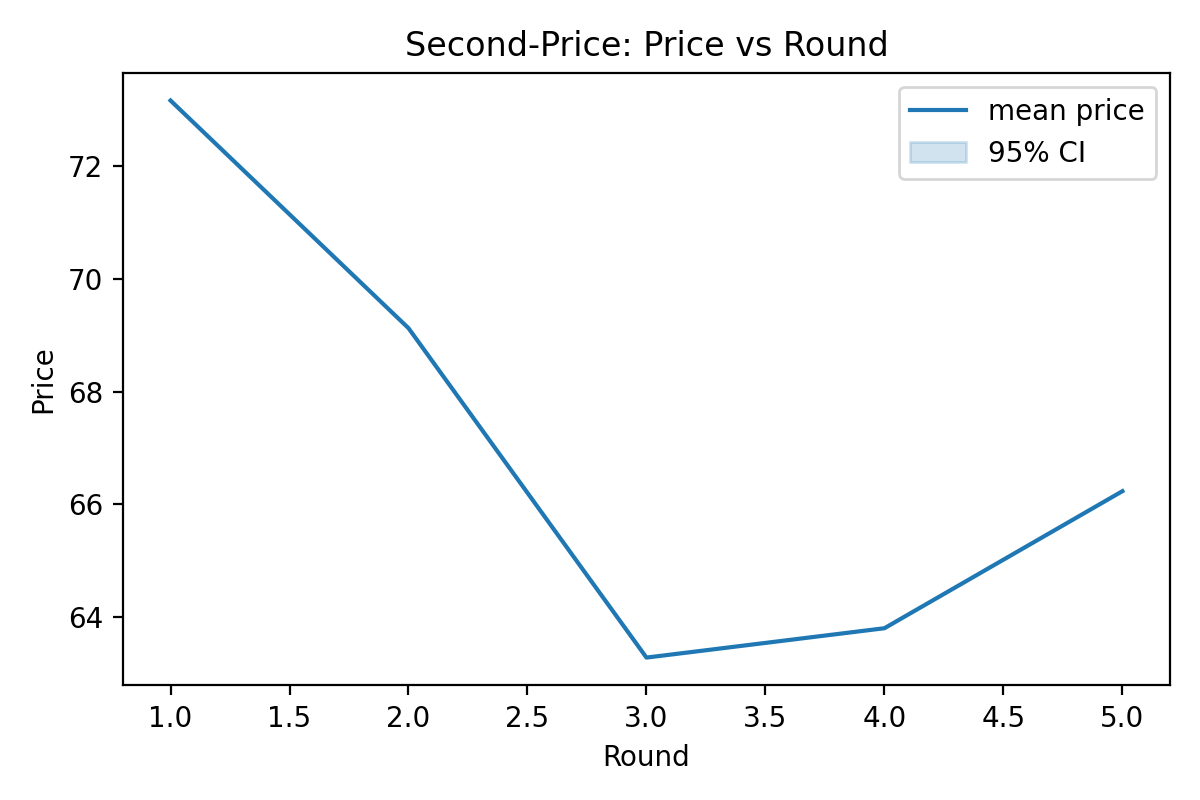
\includegraphics[width=0.75\textwidth]{figures/price_path.png}
  \caption{Average second-price by round with 95\% CIs (placeholder path).}
  \label{fig:price_path}
\end{figure}
\begin{figure}[H]
  \centering
  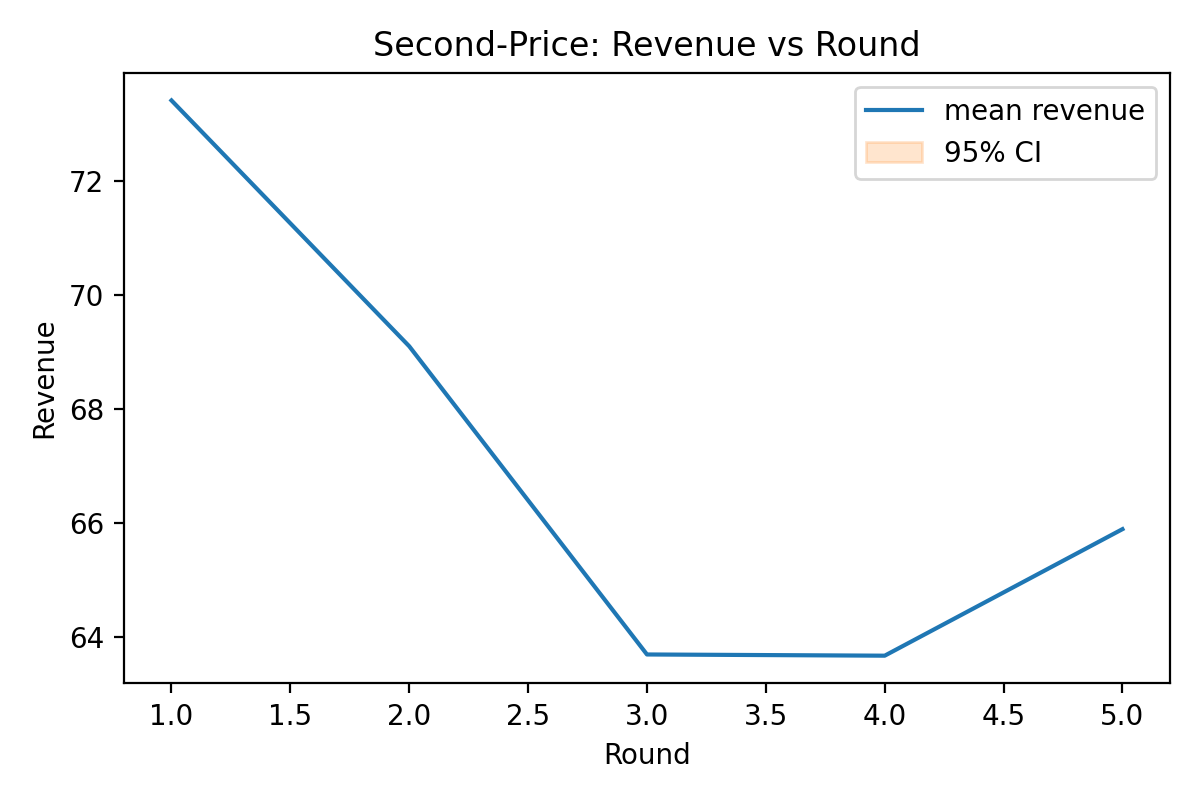
\includegraphics[width=0.75\textwidth]{figures/revenue_by_round.png}
  \caption{Seller revenue trajectory (placeholder path).}
  \label{fig:revenue_by_round}
\end{figure}
\begin{figure}[H]
  \centering
  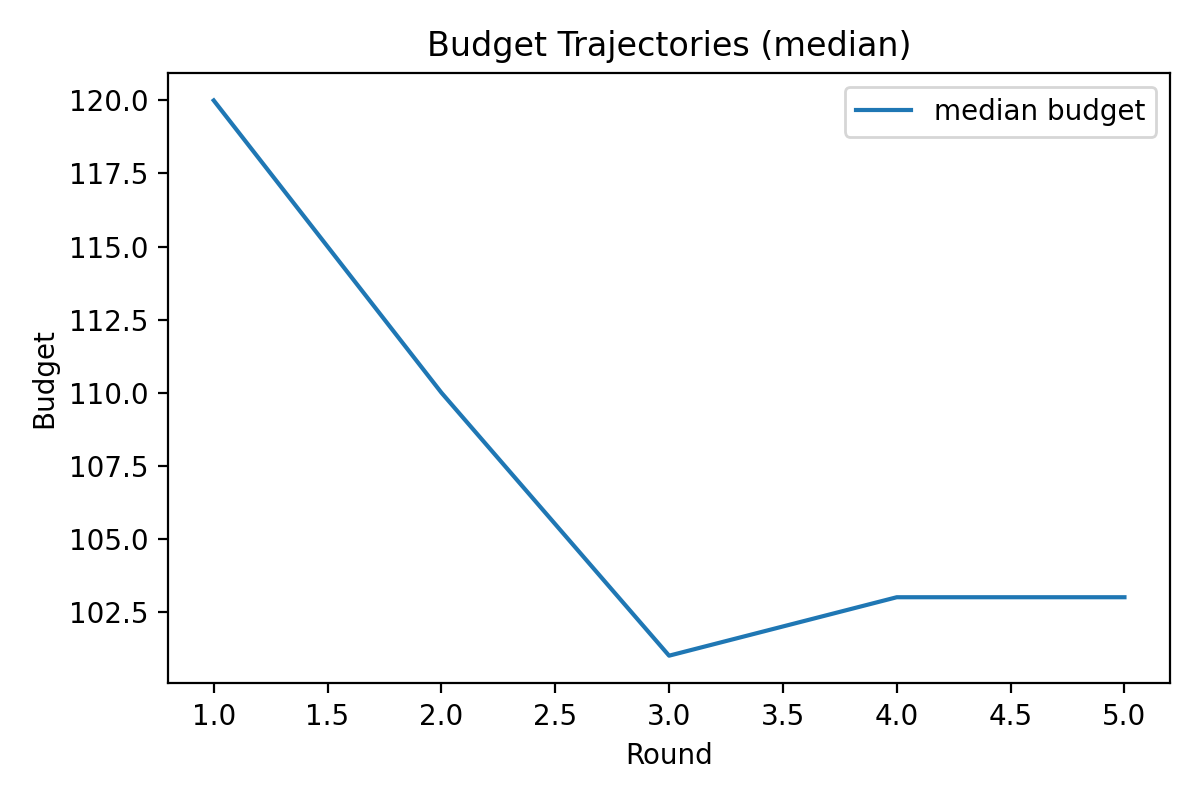
\includegraphics[width=0.75\textwidth]{figures/budget_trajectories.png}
  \caption{Median budget trajectories with bands (placeholder path).}
  \label{fig:budget_traj}
\end{figure}
\begin{figure}[H]
  \centering
  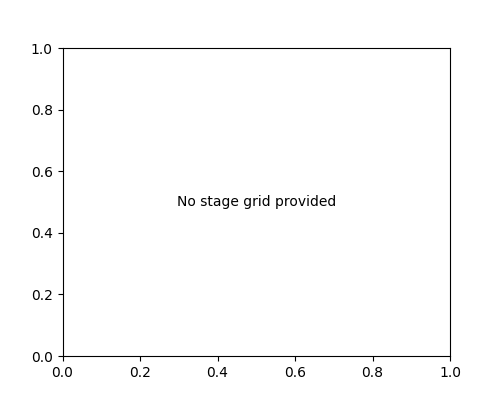
\includegraphics[width=0.75\textwidth]{figures/equilibrium_heatmap.png}
  \caption{Stage-game equilibrium heatmap over (v,B) grid (placeholder path).}
  \label{fig:eq_heatmap}
\end{figure}

\section*{Data and Code Availability}

All code used to compute equilibria, simulate threshold strategies and analyse the experimental data is available in the accompanying GitHub repository.  The dataset \texttt{all\_apps\_wide\_2025\_09\_11.csv} provided by the experimenters is included in this submission.  Bibliographic citations for \texttt{NashPy}, \texttt{QuantEcon}, \texttt{Game Theory Explorer} and \texttt{oTree} are provided in the README files of the respective subfolders.

\printbibliography

\end{document}
